\documentclass[11pt,letterpaper]{article}

\usepackage[utf8]{inputenc}
\usepackage[T1]{fontenc}
\usepackage[provide=*,spanish]{babel}
\usepackage{lmodern}
\usepackage[margin=2.25cm]{geometry}
\usepackage{xcolor}
\usepackage{graphicx}
\usepackage{booktabs}
\usepackage{tabularx}
\usepackage{longtable}
\usepackage{array}
\usepackage{hyperref}

\definecolor{navy}{HTML}{071126}
\definecolor{blue}{HTML}{2563EB}
\definecolor{cyan}{HTML}{0891B2}
\definecolor{violet}{HTML}{7C3AED}
\definecolor{green}{HTML}{15803D}
\definecolor{red}{HTML}{B42318}
\definecolor{soft}{HTML}{F1F5F9}
\definecolor{codebg}{HTML}{F7F9FC}

\hypersetup{
  colorlinks=true,
  linkcolor=blue,
  urlcolor=cyan,
  citecolor=violet,
  pdftitle={Compiscript Semantic IDE -- Proyecto 1},
  pdfauthor={DragonsSlayers 2.0}
}

\pagestyle{plain}

\renewcommand{\arraystretch}{1.2}
\newcolumntype{Y}{>{\raggedright\arraybackslash}X}
\newcommand{\archivo}[1]{\texttt{#1}}
\newcommand{\codigo}[1]{\texttt{#1}}
\newcommand{\estado}[1]{\textcolor{green}{\textbf{#1}}}

\begin{document}

\begin{titlepage}
  \pagecolor{navy}
  \color{white}
  \centering
  \vspace*{1.3cm}
  {\Large Universidad del Valle de Guatemala\par}
  \vspace{0.4cm}
  {\large Construcción de Compiladores -- CC-3032, sección 10\par}
  \vfill
  {\Huge\bfseries Compiscript Semantic IDE\par}
  \vspace{0.4cm}
  {\LARGE Proyecto 1: análisis semántico, tabla de símbolos e IDE\par}
  \vspace{1cm}
  \IfFileExists{../../presentation/assets/compiler-pipeline-hero.png}{
    
\includegraphics[width=0.86\textwidth]{../../presentation/assets/compiler-pipeline-hero.png}
  }{}
  \vfill
  {\large Grupo DragonsSlayers 2.0\par}
  \vspace{0.35cm}
  \begin{tabular}{rl}
    Pablo Daniel Barillas Moreno & 22193 \\
    Hugo Daniel Barillas Ajín & 23556 \\
    Ernesto Ascencio & 23009
  \end{tabular}
  \vspace{0.7cm}

  {\large Catedrático: Ing. Carlos Valdéz\par}
  {\large Agosto de 2026\par}
\end{titlepage}
\nopagecolor
\color{black}

\tableofcontents
\newpage

\section{Resumen ejecutivo}

Este proyecto implementa un entorno integrado para Compiscript, un subconjunto inspirado en TypeScript. La aplicación recibe código fuente, ejecuta el lexer y parser generados con ANTLR 4 y, cuando la sintaxis es válida, recorre el CST mediante un Visitor para aplicar reglas semánticas. El resultado incluye diagnósticos con ubicación, árbol semántico anotado, tabla de símbolos, árbol de ámbitos, referencias y capturas de closures.

La solución fue construida con TypeScript, React, Vite y Electron. El diseño separa el motor de compilación de la presentación: la interfaz, la CLI y las pruebas invocan el mismo orquestador. La versión final corrige problemas de identidad y alcance de clases, inferencia dependiente del orden, firmas sin retorno explícito, conteo incompleto de referencias y ejemplos incompatibles con la gramática formal.

La verificación final reporta \textbf{105 pruebas aprobadas en 6 suites}, además de compilación TypeScript y build de producción exitosos. La matriz completa se encuentra en \archivo{docs/MATRIZ\_REQUISITOS.md}.

\section{Objetivos}

\subsection{Objetivo general}

Construir una fase de análisis semántico para Compiscript que sea comprobable mediante pruebas, observable desde un IDE y suficientemente modular para servir como base de fases posteriores del compilador.

\subsection{Objetivos específicos}

\begin{enumerate}
  \item Generar el lexer y parser a partir de una gramática ANTLR.
  \item Implementar reglas de tipos, ámbitos, funciones, flujo, clases y arreglos.
  \item Construir una tabla de símbolos con inserción, recuperación, actualización y manejo de alcances.
  \item Producir un árbol semántico visual con tipos y referencias.
  \item Presentar resultados comprensibles en un IDE web y de escritorio.
  \item Mantener pruebas de éxito, fallo y regresión para las reglas requeridas.
  \item Documentar decisiones donde las fuentes del lenguaje son ambiguas.
\end{enumerate}

\section{Contexto y fuentes del lenguaje}

El desarrollo parte de tres fuentes: el README general de Compiscript, la gramática \archivo{Compiscript.g4} y el enunciado de análisis semántico. La gramática es la autoridad formal para la sintaxis; el enunciado define las validaciones; y los ejemplos ayudan a interpretar la intención del lenguaje.

Se identificaron dos discrepancias importantes:

\begin{itemize}
  \item El enunciado requiere \codigo{float}, pero la gramática base solo declara \codigo{integer}. Se añadió el token de tipo y el literal decimal como extensión mínima.
  \item El enunciado agrupa \codigo{switch} con condiciones booleanas, mientras el README muestra casos enteros y la gramática acepta una expresión general. Se adoptó un discriminante escalar y se exige comparabilidad entre discriminante y casos.
\end{itemize}

La gramática formal exige bloques con llaves para \codigo{if}, \codigo{while}, \codigo{do-while}, \codigo{for} y \codigo{foreach}. La versión activa mantiene esa restricción aun cuando algunos fragmentos narrativos del README omiten llaves.

\section{Arquitectura}

\subsection{Pipeline por fases}

\begin{figure}[htbp]
  \centering
  \IfFileExists{../../presentation/assets/compiler-pipeline-hero.png}{
    
\includegraphics[width=0.92\textwidth]{../../presentation/assets/compiler-pipeline-hero.png}
  }{
    \fbox{\parbox{0.85\textwidth}{Código fuente $\rightarrow$ lexer $\rightarrow$ parser $\rightarrow$ Visitor semántico $\rightarrow$ resultados}}
  }
  \caption{Representación conceptual del pipeline de Compiscript.}
\end{figure}

\begin{enumerate}
  \item \textbf{Lexer:} transforma caracteres en tokens y registra errores sin detener innecesariamente la exploración.
  \item \textbf{Parser:} ejecuta \codigo{program()} y produce el CST con recuperación controlada de errores.
  \item \textbf{Prepasada:} crea identidades de clase y prepara declaraciones visibles en cada ámbito.
  \item \textbf{Visitor semántico:} resuelve nombres, calcula tipos, valida reglas y construye el árbol anotado.
  \item \textbf{Presentación:} organiza un único \codigo{AnalyzeResult} para UI, CLI y exportaciones.
\end{enumerate}

La semántica queda en estado \codigo{skipped} si existen errores léxicos o sintácticos. Esto evita cascadas producidas por contextos recuperados artificialmente por el parser.

\subsection{Responsabilidades de módulos}

\begin{table}[htbp]
\centering
\begin{tabularx}{\textwidth}{>{\ttfamily}lY}
\toprule
Módulo & Responsabilidad \\
\midrule
lib/analyze.ts & Orquestación de lexer, parser, semántica y resultado común. \\
semantic/declarationVisitor.ts & Registro de clases, miembros, firmas y herencia. \\
semantic/semanticVisitor.ts & Recorrido principal del CST y construcción del árbol semántico. \\
semantic/scopes.ts & Tabla de símbolos, cadena léxica y actualización controlada. \\
semantic/typeSystem.ts & Asignabilidad, comparación, operadores e inferencia común. \\
semantic/flowAnalysis.ts & Terminación, retorno por caminos y código inalcanzable. \\
semantic/diagnostics.ts & Códigos, severidad, ubicación y deduplicación. \\
ui/ & Representación interactiva de resultados; no contiene reglas del lenguaje. \\
\bottomrule
\end{tabularx}
\caption{Separación de responsabilidades.}
\end{table}

\section{Sistema de tipos}

El modelo representa tipos primitivos, arreglos, funciones, clases, instancias, \codigo{null}, \codigo{void}, \codigo{unknown} y \codigo{error}. Los dos últimos permiten continuar el análisis sin multiplicar mensajes derivados.

\subsection{Reglas principales}

\begin{table}[htbp]
\centering
\begin{tabularx}{\textwidth}{lYY}
\toprule
Familia & Caso válido & Rechazo característico \\
\midrule
Aritmética & operandos numéricos; \codigo{string + string} & booleanos, arreglos o funciones \\
Lógica & operandos \codigo{boolean} & cualquier valor no booleano \\
Relacional & números compatibles & categorías incompatibles \\
Asignación & igualdad o promoción \codigo{integer} a \codigo{float} & conversión implícita inversa \\
Arreglos & elementos con tipo común & mezcla sin tipo compatible \\
Índice & receptor arreglo e índice entero & receptor no indexable o índice no entero \\
\bottomrule
\end{tabularx}
\end{table}

\begin{verbatim}
let contador = 1;
let promedio: float = contador;
let valores: integer[] = [1, 2, 3];
print(valores[0]);
\end{verbatim}

\subsection{Inferencia de retornos}

Una función sin anotación empieza con tipo \codigo{unknown}. Cada \codigo{return} registra el tipo observado y al terminar el cuerpo se calcula un tipo común. Una función sin retornos con valor resulta \codigo{void}. Este tratamiento evita el error previo de considerar toda función no anotada como procedimiento.

\section{Tabla de símbolos y ámbitos}

Cada símbolo almacena ID, nombre, categoría, tipo, mutabilidad, ámbito, posición de declaración, inicialización, referencias, captura y, cuando corresponde, firma o miembros.

\begin{figure}[htbp]
  \centering
  \IfFileExists{../../presentation/assets/scopes-symbol-table.png}{
    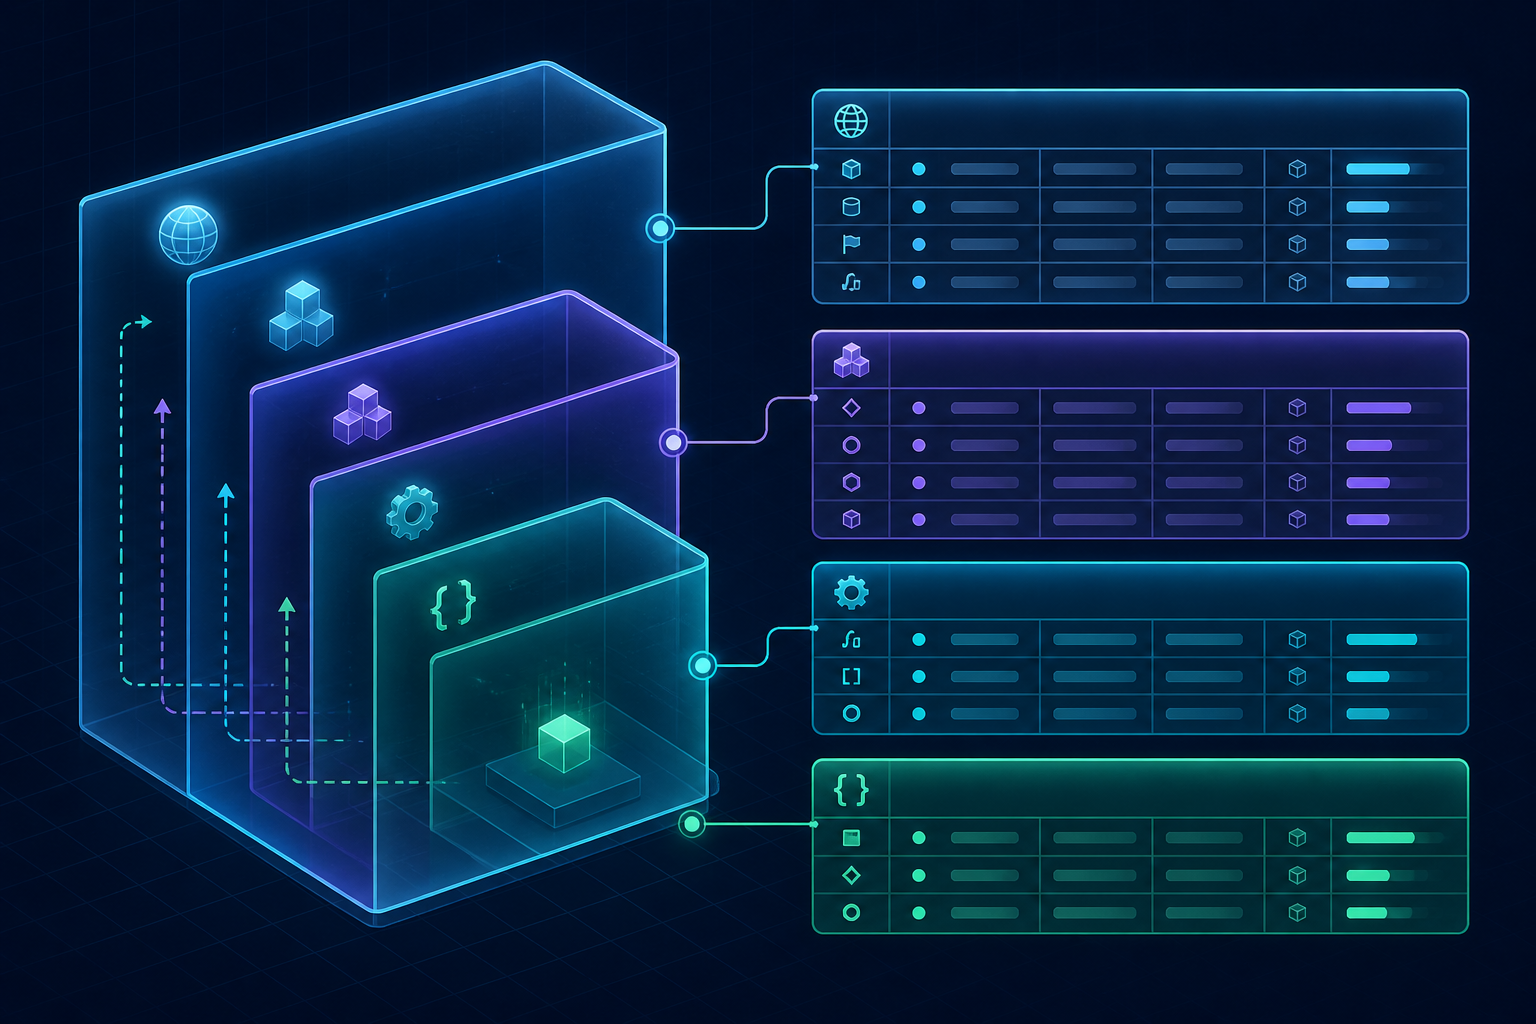
\includegraphics[width=0.88\textwidth]{../../presentation/assets/scopes-symbol-table.png}
  }{
    \fbox{\parbox{0.85\textwidth}{Ámbito global contiene ámbitos de clase, función y bloque; cada uno enlaza símbolos y referencias.}}
  }
  \caption{Modelo conceptual de ámbitos anidados y tabla de símbolos.}
\end{figure}

\subsection{Operaciones requeridas por la rúbrica}

\begin{table}[htbp]
\centering
\begin{tabularx}{\textwidth}{lYY}
\toprule
Operación & API & Garantía \\
\midrule
Insertar & \codigo{declare} & rechaza duplicados en el ámbito actual \\
Recuperar & \codigo{resolveCurrent}, \codigo{resolve} & búsqueda local o recorrido de padres \\
Actualizar & \codigo{updateSymbol} & preserva identidad y ubicación de declaración \\
Alcances & \codigo{enterScope}, \codigo{exitScope} & conserva el árbol y restaura el padre \\
\bottomrule
\end{tabularx}
\end{table}

El shadowing se permite en ámbitos hijos. La actualización controlada evita reemplazar accidentalmente el ID, el nombre o el ámbito de un símbolo. Inicialización y captura reutilizan la misma operación.

\subsection{Identidad léxica de clases}

La versión revisada eliminó el registro global por nombre. Cada declaración de clase recibe un \codigo{classId}; el nombre visible se declara en el \codigo{ScopeManager}. Los tipos de clase e instancia conservan ese ID. Por tanto, dos clases \codigo{Local} declaradas en bloques hermanos son distintas y ninguna es visible fuera de su bloque.

\section{Funciones, closures y clases}

Las funciones y clases se registran antes de recorrer las demás instrucciones del ámbito. Este hoisting local permite recursión y referencias adelantadas sin convertir las declaraciones locales en globales.

\begin{verbatim}
function factorial(n: integer): integer {
  if (n <= 1) { return 1; }
  return n * factorial(n - 1);
}

function crear(): integer {
  let base: integer = 40;
  function sumar(): integer {
    return base + 2;
  }
  return sumar();
}
\end{verbatim}

Una referencia desde una función anidada a un símbolo de una función externa marca el símbolo como capturado. La UI lo presenta en la tabla y en las métricas.

En clases se validan constructor explícito o implícito, herencia, ciclos, \codigo{this}, miembros y constantes. Los campos se recorren antes de los métodos para que la inferencia no dependa del orden textual. El árbol final recupera el orden del programa para conservar legibilidad.

\section{Control de flujo}

Las condiciones de \codigo{if} y ciclos deben ser booleanas. \codigo{return} solo es válido dentro de una función; \codigo{continue} solo dentro de ciclos; y \codigo{break} dentro de ciclos o \codigo{switch}. Las instrucciones posteriores a una terminación se reportan con \codigo{SEM018} como advertencia.

\codigo{flowAnalysis.ts} separa dos preguntas: si una instrucción termina el flujo inmediato y si una función retorna en todos los caminos. Esta separación reduce falsos positivos en bloques e instrucciones condicionales.

\section{Diagnósticos}

El catálogo comprende \codigo{SEM001} a \codigo{SEM023}; \codigo{SEM022} permanece reservado para compatibilidad y \codigo{SEM023} distingue una variable existente pero aún no inicializada. Cada mensaje contiene fase, severidad, línea, columna, descripción y sugerencia cuando aplica.

\begin{longtable}{>{\ttfamily}p{1.5cm}p{11.8cm}}
\toprule
Código & Regla \\
\midrule
\endhead
SEM001 & Identificador no declarado. \\
SEM002 & Redeclaración en el mismo ámbito. \\
SEM003 & Asignación o inicialización incompatible. \\
SEM004 & Operador aplicado a tipos inválidos. \\
SEM005 & Condición no booleana. \\
SEM006 & Cantidad incorrecta de argumentos. \\
SEM007 & Tipo de argumento incompatible. \\
SEM008 & Tipo de retorno incompatible. \\
SEM009 & Retorno fuera de una función. \\
SEM010 & \codigo{break} fuera de ciclo o \codigo{switch}. \\
SEM011 & \codigo{continue} fuera de ciclo. \\
SEM012 & Miembro inexistente. \\
SEM013 & Uso inválido de \codigo{this}. \\
SEM014 & Clase, constructor o invocación inválida. \\
SEM015 & Índice no entero. \\
SEM016 & Valor no indexable. \\
SEM017 & Arreglo heterogéneo. \\
SEM018 & Código inalcanzable. \\
SEM019 & Parámetro duplicado. \\
SEM020 & Herencia inválida o circular. \\
SEM021 & Discriminante o caso incompatible en \codigo{switch}. \\
SEM022 & Reservado para compatibilidad. \\
SEM023 & Uso antes de inicialización. \\
\bottomrule
\end{longtable}

\section{Diseño del IDE}

La refactorización visual busca que el usuario comprenda la fase antes de interpretar tablas extensas. El encabezado resume el pipeline y el estado. En semántica, una guía lateral explica el propósito de cada etapa; el editor queda como superficie principal; y los resultados se distribuyen en pestañas.

\begin{itemize}
  \item \textbf{Resumen:} métricas de salud, símbolos, referencias, ámbitos y closures.
  \item \textbf{Diagnósticos:} filtros y ubicación de cada error o advertencia.
  \item \textbf{Símbolos:} búsqueda, categorías, tipos, mutabilidad y exportación.
  \item \textbf{Ámbitos:} jerarquía navegable de entornos.
  \item \textbf{Árboles:} CST y árbol semántico comparados en una cuadrícula.
\end{itemize}

El editor incorpora carga de archivos, copia, posición del cursor, estado de preparación y atajos. Se eliminaron emojis del código y documentación; la iconografía funcional usa componentes vectoriales consistentes.

\section{Auditoría y correcciones}

\begin{longtable}{p{3.2cm}p{5.2cm}p{5.2cm}}
\toprule
Área & Hallazgo & Corrección \\
\midrule
\endhead
Clases & Registro global por nombre filtraba clases locales y chocaba con homónimos. & Identidad \codigo{classId} y resolución por tabla léxica. \\
Campos & Inferencia dependía del orden entre campos y métodos. & Campos primero; presentación restaurada al orden fuente. \\
Funciones & Falta de anotación se interpretaba como \codigo{void}. & Recolección e inferencia de retornos observados. \\
Referencias & Accesos a clase, campo y método no incrementaban todos los símbolos. & Propagación de \codigo{symbolId} y registro en cada acceso. \\
Tabla & No existía una actualización pública y verificable. & \codigo{updateSymbol} con invariantes y pruebas directas. \\
Gramática & Cuerpos de control aceptaban instrucciones sin bloque. & Reglas alineadas con \archivo{Compiscript.g4} oficial y regeneración ANTLR. \\
Ejemplos & Casos integrados conservaban \codigo{if} sin llaves. & Ejemplos y pruebas sincronizados con la gramática. \\
UI & Resultados largos competían visualmente con el editor. & Workbench, guía lateral y explorador por pestañas. \\
Documentación & Comandos desde una raíz incorrecta y cifras antiguas. & Rutas, matriz, informe y presentación actualizados. \\
\bottomrule
\end{longtable}

\section{Pruebas y resultados}

La batería incluye pruebas unitarias del \codigo{ScopeManager}, reglas semánticas, pipeline integral, ejemplos sincronizados y archivos preparados para la rúbrica.

\begin{table}[htbp]
\centering
\begin{tabular}{lr}
\toprule
Suite & Pruebas aprobadas \\
\midrule
semanticAnalyzer.test.ts & 68 \\
scopeManager.test.ts & 4 \\
analyze.compiscript.test.ts & 14 \\
rubric.examples.test.ts & 8 \\
examples.sync.test.ts & 3 \\
projectExamples.test.ts & 8 \\
\midrule
Total & \textbf{105} \\
\bottomrule
\end{tabular}
\end{table}

Los comandos finales son:

\begin{verbatim}
cd compiscript-ide-work
npm install
npm run generate
npm run check
npm test
npm run build
\end{verbatim}

En la revisión final, \codigo{npm run check}, \codigo{npm test} y \codigo{npm run build} terminaron correctamente. Vite informa una advertencia no bloqueante sobre el tamaño del bundle principal; no afecta la corrección, aunque puede mitigarse posteriormente con división dinámica de módulos.

\section{Correspondencia con la rúbrica}

\begin{table}[htbp]
\centering
\begin{tabularx}{\textwidth}{l c Y}
\toprule
Componente & Puntos & Evidencia \\
\midrule
IDE & 15 & Editor, navegación por fases, guía, resultados interactivos y exportaciones. \\
Parser y semántica & 60 & ANTLR, Visitor, sistema de tipos, 23 códigos, árbol y pruebas. \\
Tabla de símbolos & 25 & Inserción, recuperación, actualización, alcances, referencias y closures. \\
\bottomrule
\end{tabularx}
\end{table}

La contribución individual no puede inferirse desde el código final: debe demostrarse con commits reales del repositorio. No se alteró ni documentó autoría que el historial no pueda respaldar.

\section{Limitaciones y trabajo futuro}

\begin{itemize}
  \item La política de \codigo{switch} debe confirmarse con el docente debido a la contradicción entre fuentes.
  \item El bundle web puede dividirse para reducir el tamaño de descarga inicial.
  \item El análisis de retorno puede evolucionar hacia un grafo de control de flujo completo.
  \item La tabla de símbolos está preparada para alimentar una representación intermedia, pero esa fase no pertenece a esta entrega.
  \item Las referencias permiten métricas y navegación futura hacia declaración.
\end{itemize}

\section{Conclusiones}

El resultado no se limita a detectar errores: expone cómo el compilador interpreta el programa. La tabla de símbolos permite observar identidad y alcance; el árbol semántico relaciona sintaxis y tipos; los diagnósticos ofrecen evidencia localizada; y las pruebas convierten las reglas del enunciado en comportamiento reproducible.

La corrección de clases fue el cambio arquitectónico central. Separar nombre visible e identidad de declaración elimina fugas entre ámbitos y permite razonar correctamente sobre herencia e instancias. La inferencia independiente del orden y el conteo de referencias completan una representación más coherente para futuras fases.

Finalmente, la nueva interfaz presenta el pipeline de forma progresiva y evita mostrar simultáneamente todas las tablas. Junto con el informe, la matriz y la presentación HTML, la entrega queda preparada tanto para evaluación técnica como para exposición oral.

\appendix
\section{Programa breve de demostración}

\begin{verbatim}
class Caja {
  let valor = 40;

  function sumar(delta: integer) {
    return this.valor + delta;
  }
}

function ejecutar(): integer {
  let caja: Caja = new Caja();
  return caja.sumar(2);
}

print(ejecutar());
\end{verbatim}

Este programa demuestra clase, campo inferido, método sin retorno anotado, constructor implícito, invocación tipada y referencias a clase, campo y método.

\section{Documentos de la entrega}

\begin{itemize}
  \item \archivo{README.md}: ejecución, capacidades y rutas.
  \item \archivo{docs/ARQUITECTURA\_PROYECTO\_1.md}: diseño interno.
  \item \archivo{docs/DECISIONES\_SEMANTICAS.md}: políticas e inconsistencias resueltas.
  \item \archivo{docs/AUDITORIA\_PROYECTO\_1.md}: hallazgos y validación.
  \item \archivo{docs/MATRIZ\_REQUISITOS.md}: trazabilidad del enunciado.
  \item \archivo{presentation/compiscript-proyecto-1.html}: exposición interactiva.
\end{itemize}

\end{document}
